\documentclass[conference]{IEEEtran}
\IEEEoverridecommandlockouts
% The preceding line is only needed to identify funding in the first footnote. If that is unneeded, please comment it out.
\usepackage{cite}
\usepackage{amsmath,amssymb,amsfonts}
\usepackage{algorithmic}
\usepackage{graphicx}
\usepackage{textcomp}
\usepackage{xcolor}
\def\BibTeX{{\rm B\kern-.05em{\sc i\kern-.025em b}\kern-.08em
    T\kern-.1667em\lower.7ex\hbox{E}\kern-.125emX}}
\begin{document}

\title{Metodologia para mitigar o viés de similaridade nas bases de dados de MFPT e Paderborn\\
% {\footnotesize \textsuperscript{*}Note: Sub-titles are not captured in Xplore and
% should not be used}

}

\author{\IEEEauthorblockN{1\textsuperscript{st} Lucio Venturim}
\IEEEauthorblockA{\textit{dept. name of organization (of Aff.)} \\
\textit{name of organization (of Aff.)}\\
Serra, Brazil \\
lucioventurim@gmail.com}
\and
\IEEEauthorblockN{2\textsuperscript{nd} Francisco Boldt}
\IEEEauthorblockA{\textit{dept. name of organization (of Aff.)} \\
\textit{name of organization (of Aff.)}\\
Serra, Brazil \\
email address or ORCID}
\and
\IEEEauthorblockN{3\textsuperscript{rd} Given Name Surname}
\IEEEauthorblockA{\textit{dept. name of organization (of Aff.)} \\
\textit{name of organization (of Aff.)}\\
City, Country \\
email address or ORCID}
}

\maketitle

\begin{abstract}
Este artigo propõe uma metodologia para mitigar o viés de similaridade das bases Paderborn e MFPT de acordo com a separação dos dados para treinamento, validação e teste.
\end{abstract}

\begin{IEEEkeywords}
bearing, bias
\end{IEEEkeywords}

\section{Introduction}
Os processos industriais são constantemente monitorados para o fornecimento de produtos de melhor qualidade e com menores taxas de rejeição.
Porém, durante a produção podem ocorrer falhas durante os processos, que são definidas como um desvio não permitido de ao menos uma variável ou propriedade característica do sistema \cite{b1}.
Os rolamentos são indispensáveis para máquinas com partes rotativas e o monitoramento de falhas nesses componentes é importante, uma vez que 40 a 50\% das falhas de equipamentos que os possuem são causadas por falhas neles \cite{b2}.
A ``Fig.~\ref{fig1}'' ilustra os principais componentes de um rolamento.

\begin{figure}[htbp]
\centerline{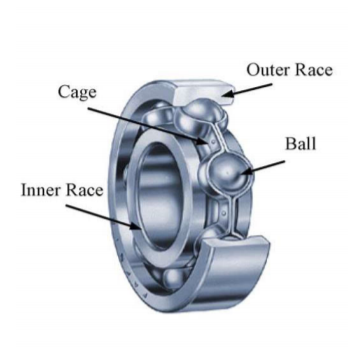
\includegraphics{artigo/fig1.png}}
\caption{Principais Elementos de um Rolamento.}
\label{fig1}
\end{figure}

O monitoramento de processos industriais pode ser dividido em quatro etapas: detecção de falhas, identificação de falhas, diagnóstico de falhas e processo de recuperação \cite{b3}.
Dentre essas etapas, o diagnóstico de falhas pode ser aplicado através de sistemas baseados em softwares, que são considerados ferramentas essenciais para garantir a segurança e manutenção de processos dinâmicos \cite{b3}.
Esses sistemas podem utilizar técnicas de aprendizado de máquina, que usam os sinais coletados de determinado equipamento para treinar e testar classificadores, e então identificar e diagnosticar as falhas \cite{b4}.

O desenvolvimento de modelos para classificação de falhas em rolamento depende da utilização de bases de dados com sinais coletados durante o funcionamento de um equipamento, que são separados em parte para treinamento e validação e parte para testes, de onde são extraídos os resultados dos experimentos.
Porém, dependendo das escolhas durante a elaboração do modelo, os experimentos podem trazer uma avaliação super otimista, onde os resultados foram adequados apenas para a configuração utilizada.
Desta forma, quando a técnica testada for aplicada na prática, possivelmente não trará resultados similares aos obtidos durante o desenvolvimento.
Uma avaliação realista deve levar em consideração a capacidade de generalização do modelo elaborado.
Assim o classificador treinado deve ser capaz de reconhecer o máximo de condições possíveis, mesmo quando há variações em suas condições de trabalho \cite{b4}.

Uma característica que influencia na capacidade de generalização de um algoritmo, de acordo com \cite{b4}, é o viés de similaridade.
O viés de similaridade ocorre quando os dados de uma mesma condição que são utilizados para o treinamento e teste do modelo têm características muito similares, tornando a tarefa de classificação relativamente trivial.
Amostras de uma mesma condição e de uma mesma aquisição, por exemplo, tipicamente são muito similares \cite{b4}.
Em \cite{b4}, são realizados experimentos com a base de dados fornecida pela Case Western Reserve University (CWRU) com diferentes formas de separação dos dados a fim de verificar a questão do viés de similaridade.
O artigo apresenta uma extensa lista de trabalhos publicados não considera esse viés no desenvolvimento de seus modelos.

As bases de dados disponibilizadas pela Machinery Failure Prevention Technology Society (MFPT) e pela Konstruktions und Antriebstechnik da Universidade de Paderborn (PADERBORN) são utilizadas para o desenvolvimento de modelos de classificação de falhas em diversos artigos.
Porém, a questão do viés de similaridade não é considerada na elaboração dos algoritmos de classificação de falhas dos artigos avaliados neste trabalho.

Uma forma de mitigar o viés de similaridade, e aumentar a capacidade de generalização de um modelo de classificação de falhas em rolamentos, é a não utilização de amostras de mesma condição e aquisição no treinamento e teste.
Para isso, deve-se definir grupos diferentes para cada aquisição e/ou outras características, para que os dados de tais grupos sejam utilizados somente para treinamento ou somente para testes.
Este artigo propõe uma metodologia para reduzir o viés de similaridade de acordo com essas regras.

A seção 2 apresenta as bases de dados MFPT e Paderborn com detalhes das bases e de artigos publicados que as utilizam.
A seção 4 descreve a metodologia utilizada para a análise do viés de similaridade das bases MFPT e Paderborn.
A seção 5 apresenta os resultados e análises dos resultados obtidos, com comparações dos resultados de outros trabalhos.
Por fim a seção 6 traz a conclusão do artigo e discute possibilidades para trabalhos futuros.

\section{Bases de Dados}

Para que a análise do viés de similaridade seja possível, é necessário que a bases de dados a ser analisada possua diferentes seções de aquisição para as diferentes condições presentes.
Para esse artigo foram utilizadas as bases MFPT e PADERBORN, que possuem essa característica.

\subsection{MFPT}

A base de dados referida como MFPT foi disponibilizada publicamente pela \textit{Machine Failure Prevention Technology Society} (MFPT).
Ela foi desenvolvida em conjunto com o trabalho \cite{b13}, que analisa um algoritmo de envelopamento e descreve técnicas para seu desenvolvimento, além de prover métodos para a determinação de uma janela otimizada para a análise dos envelopes.

A aquisição dos dados de vibração foi realizada com um aparato utilizando rolamentos NICE.
Três seções foram realizadas em condições normais, com uma carga de 270 lbs e uma frequência de aquisição de 97.656Hz por 6 segundos.
Dez seções onde os rolamentos apresentavam falha no anel externo foram executadas, três delas com uma carga de 270 lbs, também com uma frequência de aquisição de 97.656Hz por 6 segundos.
As outras sete foram realizadas com cargas de 25, 50, 100, 150, 200, 250 e 300 lbs, respectivamente, com uma taxa de amostragem de 48.828Hz por 3 segundos.
Sete seções foram realizadas com rolamentos com falhas no anel interno, com uma frequência de aquisição de 48.828Hz durante 3 segundos e cargas de 0, 50, 100, 150, 200, 250 e 300 lbs.
Além dos dados citados, são fornecidos arquivos de análises dos dados e três aquisições de situações reais (de uma turbina de vento, de uma bomba de petróleo e de um globo).
Os arquivos são disponibilizados no formato Matlab (.mat), contendo a carga, a rotação, a frequência de amostragem e um vetor com os dados de vibração.
A Tabela \ref{tab1} apresenta os tipos de falhas e as cargas das aquisições, à exceção das três aquisições de situações reais informadas.

\begin{table}[htbp]
\caption{MFPT Dataset Details}
\begin{center}
\begin{tabular}{|c|c|c|c|}
\hline
\textbf{Fault Type}&{\textbf{Load (lbs)}}&{\textbf{Sample Rate (sps)}}&\textbf{Acquisitions}\\
\hline
Health State&270&97,656&3\\
Outer Ring&270&97,656&3\\
Outer Ring&25&48,828&1\\
Outer Ring&50&48,828&1\\
Outer Ring&100&48,828&1\\
Outer Ring&150&48,828&1\\
Outer Ring&200&48,828&1\\
Outer Ring&250&48,828&1\\
Outer Ring&300&48,828&1\\
Inner Ring&0&48,828&1\\
Inner Ring&50&48,828&1\\
Inner Ring&100&48,828&1\\
Inner Ring&150&48,828&1\\
Inner Ring&200&48,828&1\\
Inner Ring&250&48,828&1\\
Inner Ring&300&48,828&1\\
\hline
\end{tabular}
\label{tab1}
\end{center}
\end{table}

A Tabela \ref{tab2} apresenta trabalhos publicados com detalhes sobre a forma de separação dos dados para o treinamento e testes dos modelos que utilizam a base de dados MFPT.

\begin{table}[htbp]
\caption{MFPT Articles Details}
\begin{center}
\begin{tabular}{|c|c|c|c|}
\hline
\textbf{Reference}&{\textbf{Splitting Strategy}}&{\textbf{Classifiers}}\\
\hline
\cite{b5}&80-20&AE, DAE, SAE, MLP, CNN\\
&&LeNet, AlexNet, ResNet18, LSTM\\
\cite{b6}&70-10-20&LCNN, ShuffleNet, ResNet\\
&&LeNet, AlexNet, TCNN\\
\cite{b7}&70-30&MLP, LSVM, SVM, CNN\\
\cite{b8}&5-fold&SECNN, CNN, CNN-VAE\\
\cite{b9}&NA&CNN\\
\hline
\end{tabular}
\label{tab2}
\end{center}
\end{table}

Em \cite{b5}, que realiza um estudo com a aplicação de métodos de aprendizado profundo em 9 bases de dados de falhas de rolamentos, incluindo a base MFPT e a Paderborn, são descritas duas formas de separação dos dados em treinamento e testes.
Uma é a separação randômica dos dados, onde as amostras são escolhidas aleatoriamente para treino e teste.
Outra é a separação pelo tempo, onde um percentual ou duração pré-definida do sinal é escolhido para treino e teste.
Em ambos os casos, são utilizadas amostras da mesma aquisição para treino e teste, e o viés de similaridade pode ocorrer.

Dentre os artigos que utilizam a base MFPT, em \cite{b6}, que propõe uma lightweight convolutional neural network (LCNN), é realizada a separação dos dados aleatoriamente com 70\% para treinamento, 10\% para validação e 20\% para teste, também utilizando amostras de mesma aquisição em todos.
\cite{b7} propõe uma metologia baseada em deep learning para aprendizado automático de características dos dados, onde a separação dos dados também foi realizada aleatoriamente com 70\% para treinamento e 30\% para teste, com amostras de mesma aquisição em ambos.
Muitos trabalhos não informam a forma de separação de dados, como em \cite{b8}, que propõe uma nova snapshot ensemble convolutional neural network (SECNN), e em \cite{b9}, que avalia o uso de convolutional neural nets (CNN) diretamente nos sinais.

\subsection{PADERBORN}

A base de dados referida como PADERBORN foi gerada e disponibilizada publicamente pela \textit{Chair of Design and Drive Technology} da Universidade Paderborn.
A base foi elaborada com o intuito de ser um \textit{benchmark} para monitoramento de condições de rolamentos no artigo \cite{b14}.
O artigo descreve detalhadamente as falhas encontradas nos rolamentos e realizados experimentos de classificação para o diagnóstico das mesmas.

O aparato para aquisição dos dados consiste de um motor elétrico, um medidor de torque, um módulo para teste de rolamentos (onde os rolamentos com diferentes condições são acopladas para geração dos dados), um volante de inércia e um motor de carga, conforme ilustrado na Figura \ref{fig2}.
No total, foram realizados experimentos com 32 rolamentos diferentes, onde 12 possuíam danos artificiais, 14 com danos obtidos em testes de tempo de duração, e 6 com rolamentos em condições normais com tempos de duração diferentes, conforme descrito na Tabela \ref{tab3}.

\begin{figure}[htbp]
\centerline{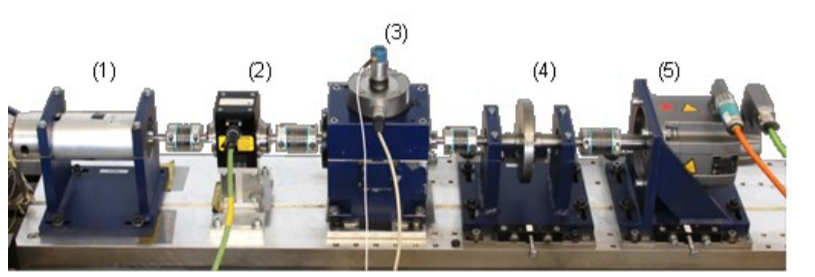
\includegraphics[height=30mm]{artigo/fig2.png}}
\caption{PADERBORN Modular Test Rig.}
\label{fig2}
\end{figure}


\begin{table}[htbp]
\caption{PADERBORN Dataset Details}
\begin{center}
\begin{tabular}{|c|c|c|}
\hline
\textbf{Bearing}&{\textbf{Fault Type}}&{\textbf{Fault Source}}\\
\hline
K001,K002,K003,&Health State&NA\\
K004,K005,K006&&\\
KA01,KA03,KA05,&Outer Ring&Artificial\\
KA06,KA07,&&\\
KA08,KA09&&\\
KI01,KI03,KI05,&Inner Ring&Artificial\\
KI07,KI08&&\\
KA04,KA15,KA16,&Outer Ring&Real\\
KA22,KA30&&\\
KA23,KA24,KA27&Outer and&Real\\
&Inner Ring&\\
KI04,KI14,KI16&Inner Ring&Real\\
KI17,KI18,KI21&&\\
\hline
\end{tabular}
\label{tab3}
\end{center}
\end{table}

Para cada rolamento, foram registrados dados para 4 diferentes condições de operação, com diferentes cargas e rotações, conforme Tabela \ref{tab4}.
20 seções de aquisição de 4 segundos cada para cada configuração foram salvas em arquivos Matlab (.mat).

\begin{table}[htbp]
\caption{PADERBORN Operating Parameters}
\begin{center}
\begin{tabular}{|c|c|c|c|}
\hline
\textbf{Setting}&{\textbf{Rotational}}&{\textbf{Load}}&{\textbf{Radial}}\\
 \textbf{No.}&\textbf{Speed (RPM)}&\textbf{Torque (Nm)}&\textbf{Force (N)}\\
\hline
1&1500&0.7&1000\\
2&900&0.7&1000\\
3&1500&0.1&1000\\
4&1500&0.7&400\\
\hline
\end{tabular}
\label{tab4}
\end{center}
\end{table}

A Tabela \ref{tab5} apresenta trabalhos publicados com detalhes sobre a forma de separação dos dados para o treinamento e testes dos modelos que utilizam a base de dados PADERBORN.

\begin{table}[htbp]
\caption{PADERBORN Articles Details}
\begin{center}
\begin{tabular}{|c|c|c|c|}
\hline
\textbf{Reference}&{\textbf{Splitting Strategy}}&{\textbf{Classifiers}}\\
\hline
\cite{b5}&80-20&AE, DAE, SAE, MLP, CNN\\
&&LeNet, AlexNet, ResNet18, LSTM\\
\cite{b10}&60-20-20&MLP, SVM, DBN, CNN, IFM\\
\cite{b11}&Arbitrary&ACDIN, DIN, ACCNN\\
\cite{b12}&80-10-10&SVC, KNN, ACDIN, WDCNN\\
&&AlexNet, ResNet, ICN\\
\cite{b14}&5-fold&CART, RF, BT, NN,\\
&&SVM-PSO, ELM, KNN\\
\hline
\end{tabular}
\label{tab5}
\end{center}
\end{table}

Para os artigos onde a base Paderborn é utilizada, alguns utilizam dados de mesma aquisição tanto para o treinamento como para o teste como ocorre no já citado \cite{b5}.
Entre eles \cite{b10}, que propõe uma deep residual network (ResNet) baseada em input feature mappings (IFMs).
Outros artigos realizam experimentos onde não são utilizados dados de mesma aquisição para treino e teste simultaneamente, como em \cite{b11}, que propõe uma deep inception net com atrous convolution (ACDIN) para tratar do problema de utilizar dados de danos artificiais com mais confiabilidade, e em \cite{b12}, que propõe uma nova capsule network.
Para esses casos, a separação não considerando a aquisição não foi com o objetivo explícito de evitar algum viés de similaridade.
Porém, para a base PADERBORN, o viés de similaridade pode ocorrer não somente pela utilização de mesma aquisição, mas também de outras formas, como dados de mesmo rolamento com mesma carga, ou até de mesmo rolamento, a ser confirmado com a metodologia deste trabalho.

\section{Metodologia}

O viés de similaridade, conforme \cite{b4} ocorre quando os dados utilizados para treinamento têm características muito similares com aqueles utilizados para testes. 
Essa similaridade pode ocorrer, por exemplo, devido aos dados serem provenientes de uma mesma seção de aquisição.
Porém, dependendo de outros fatores, mesmo dados de aquisições diferentes podem possuir alto grau de similaridade.
Nesses casos, para mitigar o viés de similaridade, é necessário considerar outras características quando da separação dos dados, como a carga, por exemplo.

A definição de grupos de acordo com a aquisição, ou com outras características, é o primeiro passo no processo para mitigar o viés de similaridade.
Com a definição de grupos diferentes, as regras de separação dos dados em treinamento e testes devem considerar que os dados de um mesmo grupo não podem constar para treinamento e para testes simultaneamente.


\section{Experimentos}

Os experimentos foram realizados para as bases MFPT e PADERBORN considerando as regras da metodologia.
Os algoritmos escolhidos foram os mais utilizados nos artigos citados, assim como a forma de separação dos dados.

Normalização.
Forma de entrada (tempo, frequencia, heterogeneous).


\subsection{MFPT}

Descrever os resultados obtidos para os experimentos, com as diferentes divisões entre treinamento, validação e teste.



\subsection{PADERBORN}

Descrever os resultados obtidos para os experimentos, com as diferentes divisões entre treinamento, validação e teste.

\section{Comparação de Resultados}

Comparativo dos resultados a fim de corroborar o viés de similaridade.

\section{Conclusões}

Conclusão.


\section*{Acknowledgment}

The preferred spelling of the word ``acknowledgment'' in America is without 
an ``e'' after the ``g''. Avoid the stilted expression ``one of us (R. B. 
G.) thanks $\ldots$''. Instead, try ``R. B. G. thanks$\ldots$''. Put sponsor 
acknowledgments in the unnumbered footnote on the first page.


\begin{thebibliography}{00}
\bibitem{b1} Isermann, Rolf, and Peter Balle. "Trends in the application of model-based fault detection and diagnosis of technical processes." Control engineering practice 5.5 (1997): 709-719.
\bibitem{b2} Nandi, Subhasis, Hamid A. Toliyat, and Xiaodong Li. "Condition monitoring and fault diagnosis of electrical motors—A review." IEEE transactions on energy conversion 20.4 (2005): 719-729.
\bibitem{b3} Chiang, Leo H., Evan L. Russell, and Richard D. Braatz. Fault detection and diagnosis in industrial systems. Springer Science and Business Media, 2000.
\bibitem{b4} Rauber, Thomas Walter, et al. "An experimental methodology to evaluate machine learning methods for fault diagnosis based on vibration signals." Expert Systems with Applications (2020): 114022.
\bibitem{b5} Zhao, Zhibin, et al. "Deep learning algorithms for rotating machinery intelligent diagnosis: An open source benchmark study." ISA transactions 107 (2020): 224-255.
\bibitem{b6} Wang, Yanxin, et al. "Bearing intelligent fault diagnosis in the industrial Internet of Things context: A lightweight convolutional neural network." IEEE Access 8 (2020): 87329-87340.
\bibitem{b7} Verstraete, David, et al. "Deep learning enabled fault diagnosis using time-frequency image analysis of rolling element bearings." Shock and Vibration 2017 (2017).
\bibitem{b8} Wen, Long, Liang Gao, and Xinyu Li. "A new snapshot ensemble convolutional neural network for fault diagnosis." Ieee Access 7 (2019): 32037-32047.
\bibitem{b9} Lee, Dean, et al. "Convolutional neural net and bearing fault analysis." Proceedings of the International Conference on Data Science (ICDATA). The Steering Committee of The World Congress in Computer Science, Computer Engineering and Applied Computing (WorldComp), 2016.
\bibitem{b10} Hou, Liangsheng, et al. "Input Feature Mappings-Based Deep Residual Networks for Fault Diagnosis of Rolling Element Bearing With Complicated Dataset." IEEE Access 8 (2020): 180967-180976.
\bibitem{b11} Chen, Yuanhang, et al. "ACDIN: Bridging the gap between artificial and real bearing damages for bearing fault diagnosis." Neurocomputing 294 (2018): 61-71.
\bibitem{b12} Zhu, Zhiyu, et al. "A convolutional neural network based on a capsule network with strong generalization for bearing fault diagnosis." Neurocomputing 323 (2019): 62-75.
\bibitem{b13} Bechhoefer, Eric. "A quick introduction to bearing envelope analysis." Green Power Monit. Syst (2016).
\bibitem{b14} Lessmeier, Christian, et al. "Condition monitoring of bearing damage in electromechanical drive systems by using motor current signals of electric motors: A benchmark data set for data-driven classification." Proceedings of the European conference of the prognostics and health management society. 2016.
\end{thebibliography}
\vspace{12pt}

\end{document}
